%!TEX root = /Users/gijs/Work/sonic-gesture/thesis/thesis.tex
\chapter{Body Part Detection}
\label{ch:bodyparts}


\section{Face detection - Haar classifier}
Finding faces in a image is a rather well solved problem. Faces are easy to detect, first of all because people don't tilt their head often, or not more than a couple degrees. This results in that in most movies and pictures the head of a subject is up right. Also a face has easy to detect features like eyes, eyebrows, a mouth and nose. When comparing different faces, these features are - with a small variation - on the same distance and orientation.

Detecting faces is done using the haar classifier, a  boosted rejection cascade that is trained with Haar-like wavelet features\cite{Lienhart02anextended}.
Haar wavelets, histogram building.


\section{Color space conversion}
Usually pixel values of a image are stored in the Red, Green Blue (RGB) format. Advantages can be gained by converting this color space into an other, for example Hue, Saturation, Value (HSV). The HSV space splits out hue (color) from saturation (how .. is) and brightness (how .. is).

\begin{figure}[htbp]
	\center
	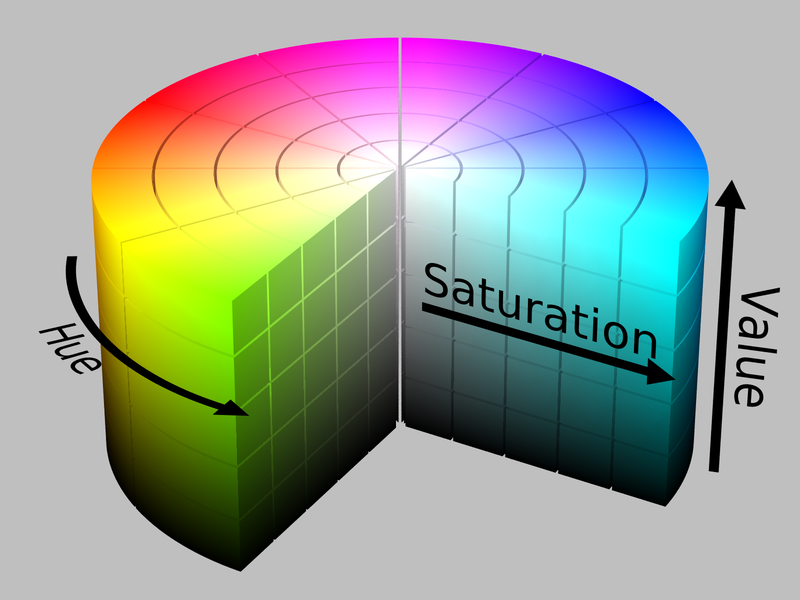
\includegraphics[width=0.4\linewidth]{figures/hsv.png}
	\caption{The Hue, Saturation, Value color space}
	\label{fig:hsv}
\end{figure}



HSV space separates out hue (color) from saturation (how concentrated the color is) and from brightness. We create our color models by taking 1D histograms from the H (hue) channel in HSV space.


 The RGB color space is transformed into the HSI color space using the following equations:

\begin{eqnarray*}
	V&\leftarrow \max(R,G,B) \label{first} \\
	S&\leftarrow \{
\end{eqnarray*}



\section{Skin color histogram}
When a face is found a color model for the subjects skin can be created. this is done by constructing a 2 dimensional histogram with the Hue and Saturation values. The optimal number of bins can't be exactly determined, a not to high or not to low value is important. 
Sonic Gesture used 180 bins for Hue and 256 for Saturation. \marginpar{EXPERIMENT WITH THIS}

\section{Blob detection}
Back projection, morphological transformations

\section{Pixel grouping, contour extraction}
join touching pixels

\section{Blob labeling}
Heuristics for blob labeling

\section{Blob label stabilization}
Kalman filter (prediction) and template search

\section{Discussion}
Ignoring the Value channel in the HSV color space to make the system invariant for lighting intensity changes assumes that the light source is pure white - a saturation of zero. In reality this is never the case, since creating artificial light that is pure white is difficult to accomplish, if not impossible.